
%(BEGIN_QUESTION)
% Copyright 2006, Tony R. Kuphaldt, released under the Creative Commons Attribution License (v 1.0)
% This means you may do almost anything with this work of mine, so long as you give me proper credit

Analyze the following electronic thermal conductivity sensor, used to detect different chemical components exiting the column of a chromatograph.  Both the measurement and reference filaments are heated by the electric current going through them, and a varying voltage will develop across each one as each is cooled differently by the gases:

$$\includegraphics[width=15.5cm]{i00678x01.eps}$$

Explain the following things about this circuit:

\begin{itemize}
\item{} How does the rheostat adjust current equally through {\it both} filaments?
\item{} How do opamp $U_1$ and transistor $Q_1$ work together to regulate current through the measurement filament?
\item{} How can we tell that opamp $U_1$ is truly functioning in negative-feedback mode, since at first glance it looks like positive feedback with the $R_{shunt}$ voltage signal connecting to the noninverting (+) input?
\item{} What is the function of opamp $U_2$ and its four equal-value resistors?
\item{} Where would an output voltage signal be measured in this circuit?
\item{} Which direction does the output voltage signal go when the measurement filament heats up to a greater temperature, assuming a positive temperature coefficient of resistance ($\alpha$) for the filament metal?
\end{itemize}

\underbar{file i00678}
%(END_QUESTION)





%(BEGIN_ANSWER)

\begin{itemize}
\item{} How does the rheostat adjust current equally through {\it both} filaments?  {\it The rheostat adjusts current through the reference filament, which then acts as a setpoint for the measurement filament circuit.}
\vskip 10pt
\item{} How do opamp $U_1$ and transistor $Q_1$ work together to regulate current through the measurement filament? {\it Opamp $U_1$ senses the voltage dropped by both shunt resistors and tries to keep them equal, resulting in equal current through both filaments.}
\vskip 10pt
\item{} How can we tell that opamp $U_1$ is truly functioning in negative-feedback mode, since at first glance it looks like positive feedback with the $R_{shunt}$ voltage signal connecting to the noninverting (+) input? {\it If the current through the measurement filament grows too large, the voltage drop across the right-hand $R_{shunt}$ will exceed the voltage drop across the other shunt resistor.  This will make the noninverting input less positive than the inverting input, driving the output of $U_1$ in the negative direction.  This will tend to turn $Q_1$ off, decreasing the measurement filament's current and bringing it closer to equality with the reference filament current.}
\vskip 10pt
\item{} What is the function of opamp $U_2$ and its four equal-value resistors? {\it This is a differential voltage amplifier with a voltage gain of 1 (0 dB).}
\vskip 10pt
\item{} Where would an output voltage signal be measured in this circuit? {\it At the output of $U_2$.}
\vskip 10pt
\item{} Which direction does the output voltage signal go when the measurement filament heats up to a greater temperature, assuming a positive temperature coefficient of resistance ($\alpha$) for the filament metal? {\it Assuming identical filaments, the output voltage will be zero when both filaments are at the same temperature, and it will drive negative when the measurement filament grows hotter than the reference filament.}
\end{itemize}


%(END_ANSWER)





%(BEGIN_NOTES)

$$\includegraphics[width=15.5cm]{i00678x02.eps}$$

\filbreak \vskip 20pt \vbox{\hrule \hbox{\strut \vrule{} {\bf Virtual Troubleshooting} \vrule} \hrule}

\noindent
{\bf Predicting the effect of a given fault:} present each of the following faults to the students, one at a time, having them comment on all the effects each fault would produce.

\begin{itemize}
\item{} 
\item{} 
\item{} 
\end{itemize}


\vskip 10pt


\noindent
{\bf Identifying possible/impossible faults:} present symptoms to the students and then have them determine whether or not a series of suggested faults could account for all the symptoms, explaining {\it why} or {\it why not} for each proposed fault:

\begin{itemize}
\item{} Symptom: {\it }
\item{}  -- {\bf Yes/No}
\item{}  -- {\bf Yes/No}
\item{}  -- {\bf Yes/No}
\end{itemize}


\vskip 10pt


\noindent
{\bf Determining the utility of given diagnostic tests:} present symptoms to the students and then propose the following diagnostic tests one by one.  Students rate the value of each test, determining whether or not it would give useful information (i.e. tell us something we don't already know).  Students determine what different results for each test would indicate about the fault, if anything:

\begin{itemize}
\item{} Symptom: {\it $V_{out}$ is ``pegged'' fully positive}
\item{} Measure $V_{JH}$ -- {\bf No}
\item{} Measure $V_{CH}$ -- {\bf Yes}
\item{} Measure $V_{DH}$ -- {\bf Yes}
\item{} Measure $V_{JA}$ -- {\bf Yes}
\item{} Measure $V_{JB}$ -- {\bf Yes}
\item{} Measure $V_{EF}$ -- {\bf Yes}
\end{itemize}


\vskip 10pt


\noindent
{\bf Diagnosing a fault based on given symptoms:} imagine the ??? fails ??? in this system (don't reveal the fault to students!).  Present the operator's observation(s) to the students, have them consider possible faults and diagnostic strategies, and then tell them the results of tests they propose based on the following symptoms, until they have properly identified the nature and location of the fault:

\begin{itemize}
\item{} Operator observation: {\it }
\item{} 
\item{} 
\end{itemize}
%INDEX% Measurement, analytical: chromatography

%(END_NOTES)


